\documentclass[a4paper,9pt,twocolumn]{extarticle}
\usepackage[utf8]{inputenc}
\usepackage{graphicx}
\usepackage[center]{caption}
\usepackage[english]{babel}
\usepackage[top=2.5cm, bottom=2.5cm, left=2.5cm, right=2.5cm]{geometry}

%---------------------------------------------
% Font packages
%---------------------------------------------
\usepackage{lmodern}
% \usepackage{concmath}
% \usepackage{cmbright}
% \usepackage{kpfonts}
% \usepackage[adobe-utopia]{mathdesign}
% \usepackage{fouriernc}
\usepackage[T1]{fontenc}

%---------------------------------------------
% Math environment packages & command
%---------------------------------------------
\usepackage{amsmath}
\usepackage{amssymb}
\usepackage{array}
% \usepackage{mathrsfs}
\usepackage{array}
% \def\sgn{\mathop{\rm sgn}\nolimits} 
% \usepackage{bbm}


%---------------------------------------------
% item option
%---------------------------------------------
\renewcommand{\labelitemi}{-}


%---------------------------------------------
%HEADER & FOOTER
%---------------------------------------------
\usepackage{fancyhdr}
\pagestyle{fancy}

\renewcommand{\headrulewidth}{.15pt}
\fancyhead[C]{{\textsc{Classical Loop-Shaping}}} 
\fancyhead[L]{Page \thepage \ of \pageref{LastPage}}
\fancyhead[R]{EL2520}

\renewcommand{\footrulewidth}{.15pt}
\fancyfoot[C]{\thepage} 
% \fancyfoot[L]{truc}
\fancyfoot[R]{EE -- Automatic Control}

\usepackage{lastpage}

%---------------------------------------------
% two column option
%---------------------------------------------
%\setlength{\columnsep}{1cm}

%---------------------------------------------
% Table of content
%---------------------------------------------
\usepackage[colorlinks,linkcolor=black, citecolor=black]{hyperref}

%---------------------------------------------
% Opening
%---------------------------------------------
\title{Computer Exercice:\\ \textsc{Classical Loop-Shaping}}
\author{Jean-Alix \textsc{David}, Kilian \textsc{Demeulemeester} \\ \texttt{\{jadavid,kiliande\}@kth.se}}

%---------------------------------------------
% Numerotation Handling
%---------------------------------------------
\setcounter{section}{3}
\usepackage[explicit]{titlesec}
% \titleformat{<command>}[<shape>]{<format>}{<label>}{<sep>}{<before>}[<after>]
\titleformat{\subsubsection}[hang]{\Large\normalsize\bfseries\centering}%
    {}{4pt}%
    {\emph{#1 \arabic{section}.\arabic{subsection}.\arabic{subsubsection}}} 
    \titleformat{\paragraph}[hang]{\footnotesize\bfseries\centering}{}{4pt}{\emph{#1}}

%---------------------------------------------
% Dummy text
%---------------------------------------------
\usepackage{lipsum}
%---------------------------------------------
% Item package option 
%---------------------------------------------
\usepackage{enumitem}
\begin{document}

% Indent length
\setlength\parindent{0em}
\setlength\itemsep{0pt}
\setlength\parskip{0pt}
\setlength\parsep{0pt}

\maketitle

%\tableofcontents

\begin{bfseries}
\emph{Abstract} -- Blablabla ! 
\end{bfseries}


\section{Exercises}

\subsection{Basics}

We consider a system which can be modeled by the transfer function:

$$ G(s) = \frac{3(-s+1)}{(5s+1)(10s+1)} $$

\subsubsection{Exercise}

We want to design a lead-lag controller which eliminates the static control error for a step response in the reference signal.

The controller transfer function is the following:

$$ F(s) = K \frac{\tau_D s + 1}{\beta \tau_D s + 1} \frac{\tau_I s + 1}{\tau_I s + \gamma}$$

We want to fulfill the following criteria:
\begin{itemize}
 \item Phase margin of $30^{\circ}$ at the cross-over frequency $\omega_c = 0.4$ rad/s.
 \item No static control error for a step response 
\end{itemize}

\subsubsection{Exercise} 

The main differences between the minimum phase case and the non-minimum phase case using a decentralized controller are:
\begin{shortitemize}
    \item The non-minimum phase system is much slower (both for step response and disturbance rejection);
    \item The step response of the non-minimum phase system starts by decreasing its value (wrong direction!);
    \item Disturbances on the top tanks have more impact on the non-minimum phase system (whereas the perturbation on the lower tanks have a similar impact on both systems).
\end{shortitemize}


\subsubsection{Exercise}

Using the method depicted in Exercice \ref{exo411} with $\tau_I = 1$s places the integral action too close to the cross-over frequency: The lag-action and the lead-action of the controller are overlapping.

Therefore, we increase the value of $\tau_I$ to $\tau_I = 10$s.

The resulting controller fulfill all the criteria. (see Figure \ref{figbode413} and \ref{figstep413}).

The lead lag controller with a phase-margin of $50^{\circ}$ has the following caracteristics:
\begin{center}
\begin{tabular}{|c|c|}
    \hline
    Bandwith ($-3dB$) & $[0,0.99]$(rad/s)\\
    \hline
    Resonance peak $M_T$ & $2.06$dB at $0.56$(rad/s)\\
    \hline
    Rise time $t_r$ & $2.22$ s\\
    \hline
    Overshoot $D$\% & $15.7$\%\\
    \hline
\end{tabular}
\end{center}

\begin{figure}[h!t]
   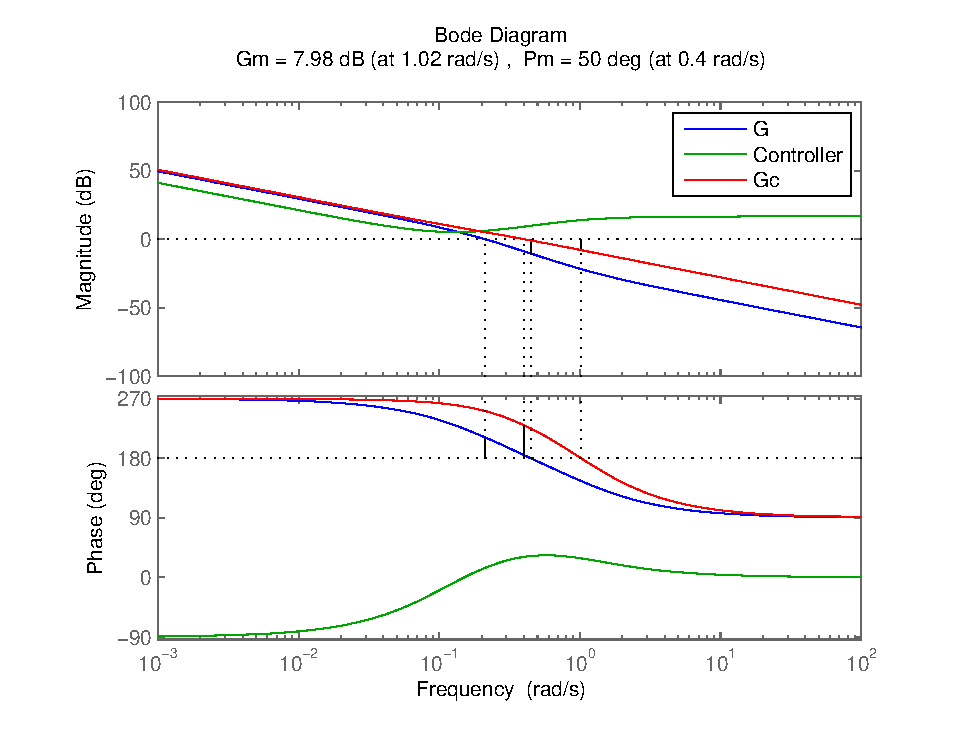
\includegraphics[width=\columnwidth]{fig/bode413.eps}
    \caption{Bode diagram of the system's functions \\ Phase-margin: $50^{\circ}$} 
    \label{figbode413}
\end{figure}

\begin{figure}[h!t]
   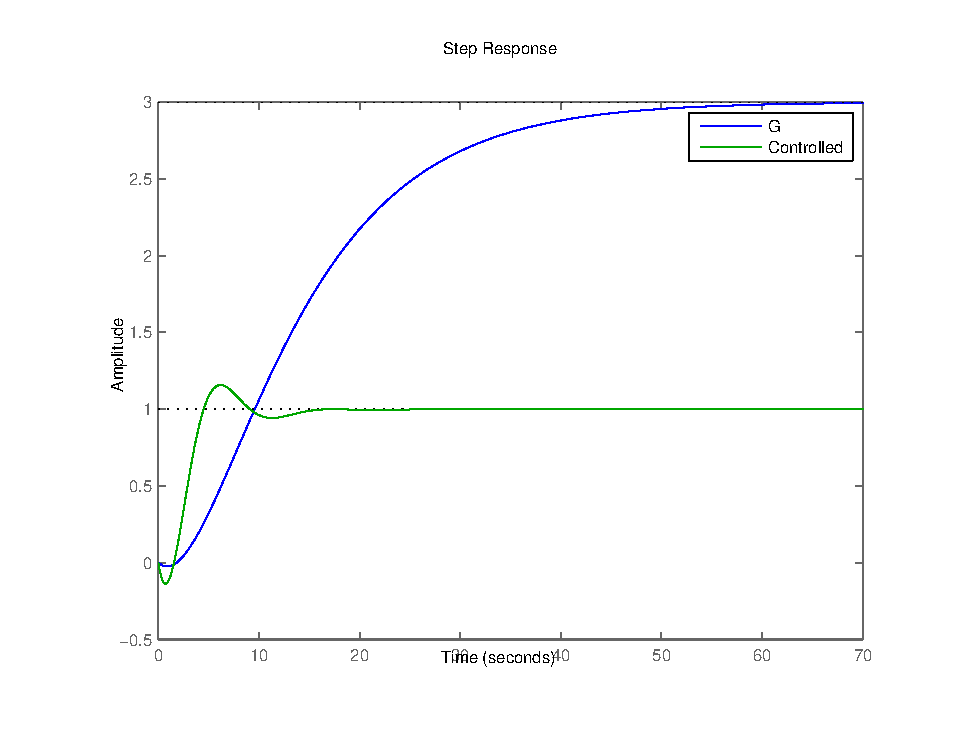
\includegraphics[width=\columnwidth]{fig/step413.eps}
    \caption{Step response of the system with and without the controller \\ Phase-margin: $50^{\circ}$}
    \label{figstep413}
\end{figure}






\subsection{Disturbance attenuation}

In this subsection, we need to design a controller which both tracks the reference signal and attenuates the disturbances. 

The transfer function of the system is:

$$G(s) = \frac{20}{(s+1)((\frac{s}{20})^2+\frac{s}{20}+1)}$$

The disturbance transfer function is:

$$G_d(s) = \frac{10}{s+1}$$

The purpose of this subsection is to designed the prefilter function and the feedback function ($F_r$ and $F_y$) with the following specifications:

\begin{itemize}
    \item Rise time $t_r \leq 0.2$ s
    \item Overshoot $D(\%) \leq 10\%$
    \item Step in the disturbance:
        $$|y(t)| \leq 1, \forall t \text{ and } |y(t)| \leq 0.1, \forall t \geq 0.5\text{ s}$$ 
    \item Control signal obeys:
        $$|u(t)| \leq 1, \forall t$$
\end{itemize}

\subsubsection{Exercise}

Since $G_d(s) = \frac{10}{s+1}$, the cross-over frequency is $w_c = 10$ rad/s.

We have the following result:

$$\forall \omega < \omega_c, |Gd(j\omega)| >1$$

Control action is needed at least for $\omega \in [0,\omega_c]$.

Here, we will try to design $F_y$ in such a way that:
$$L(s) = F_y G \approx \frac{\omega_c}{s}$$

\paragraph{Unproper feedback}
Let:
$$F_y = G^{-1} \frac{\omega_c}{s} = \frac{200 s^3 + 4200 s^2 + 84000 s + 80000}{160000 s}$$

This controller has $3$ zero and $1$ pole. Thus, it is not proper. However -- using \texttt{Matlab} -- we can plot the step response of the system and the step response to a step perturbation (see Figure \ref{stepNonProper}).

\begin{figure}[h!t]
    \centering
    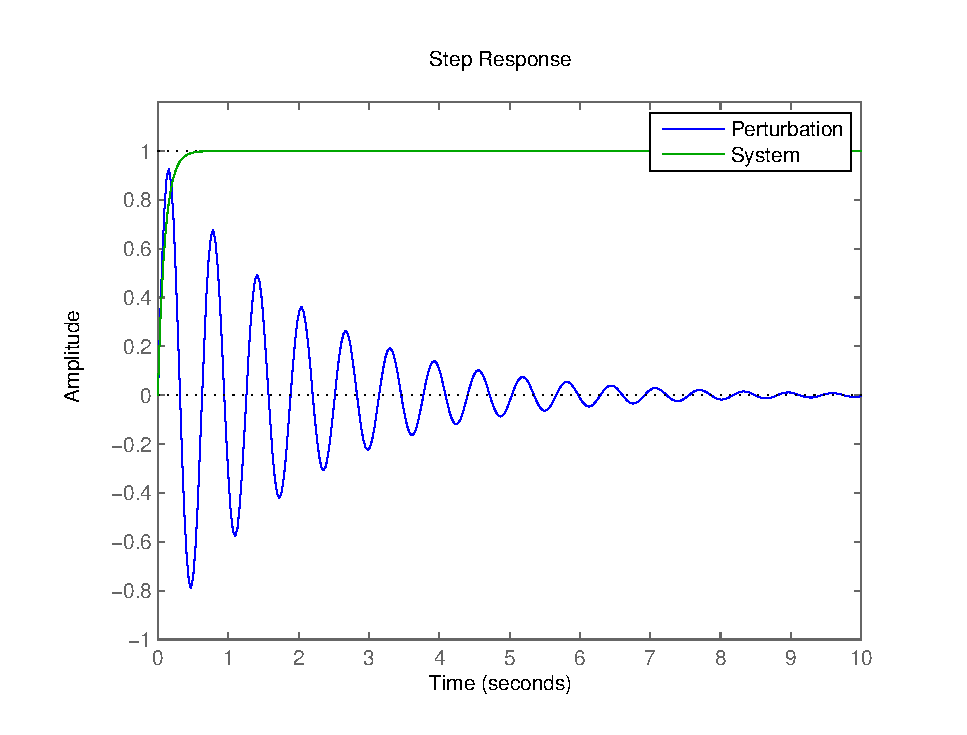
\includegraphics[width=\linewidth]{fig/stepNonProper421.eps}
    \caption{Non-proper step response of the system}
    \label{stepNonProper}
\end{figure}

We can see that even if the performance are poor (Error static $\leq 5\%$ for $t \geq t_d = 7$ s) we still have an attenuation of the perturbation and a step response of good quality.

\paragraph{Proper feedback}
Assuming that this controller is the one we want to implement, we need to design it in a proper way. For now, it has $3$ zeros and $1$ pole. Therefore it is needed to add two more poles.

Let:
$$F_y(s) = G^{-1}\frac{\omega_c}{s(s+p_1)(s+p_2)}$$

We need to choose $p_{1,2}$ in order to not change the system performance two much.

We use the following criteria:

\begin{shortitemize}
    \item $p_1 = p_2$
    \item $p_1$ and $p_2$ take action after $\omega_c$ 
\end{shortitemize}

Let's pick $p_1 = p_2 = p = 100\omega_c$. In order to have the same bode diagram for $\omega < \omega_c$, we need to translate the gain curve with a gain of $p^2$. Figure \ref{bodeProper421} shows the bode diagram of $L(s) = F_y(s) G(s)$ (we can see that $\forall \omega < \omega_c, |L_{proper}|_{dB} \approx |L_{unproper}|_{dB}$). Figure \ref{stepProper421} shows that the step response to a perturbation with $L_{proper}$ is almost the same than with $L_{unproper}$.

\begin{figure}[h!b]
    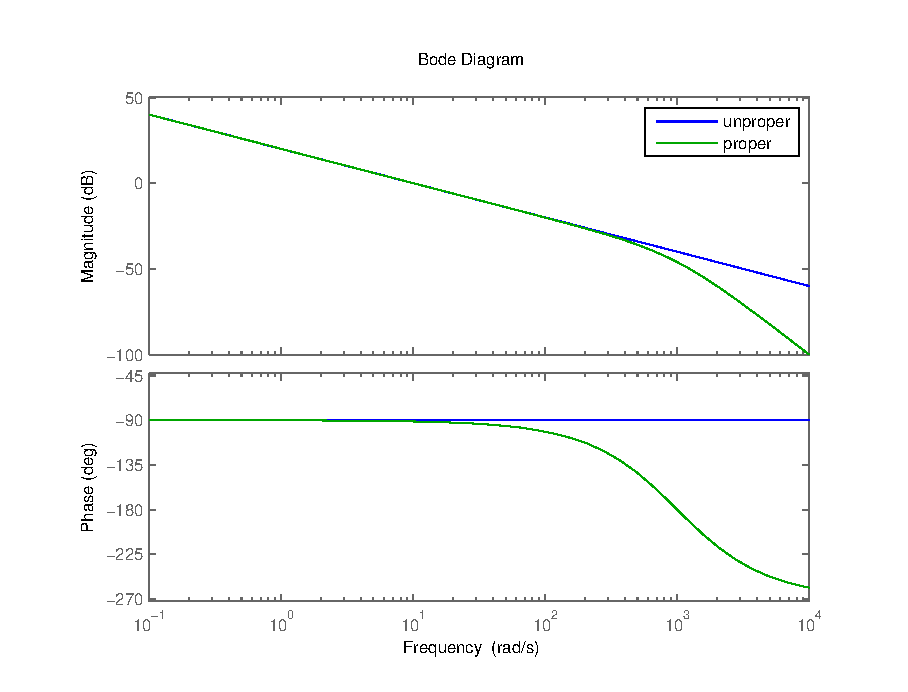
\includegraphics[width=\columnwidth]{fig/bodeProper421.eps}
    \caption{Bode diagram of $L(s)$ with the proper \& unproper $F_y$} 
    \label{bodeProper421}
\end{figure}

\begin{figure}[h!b]
    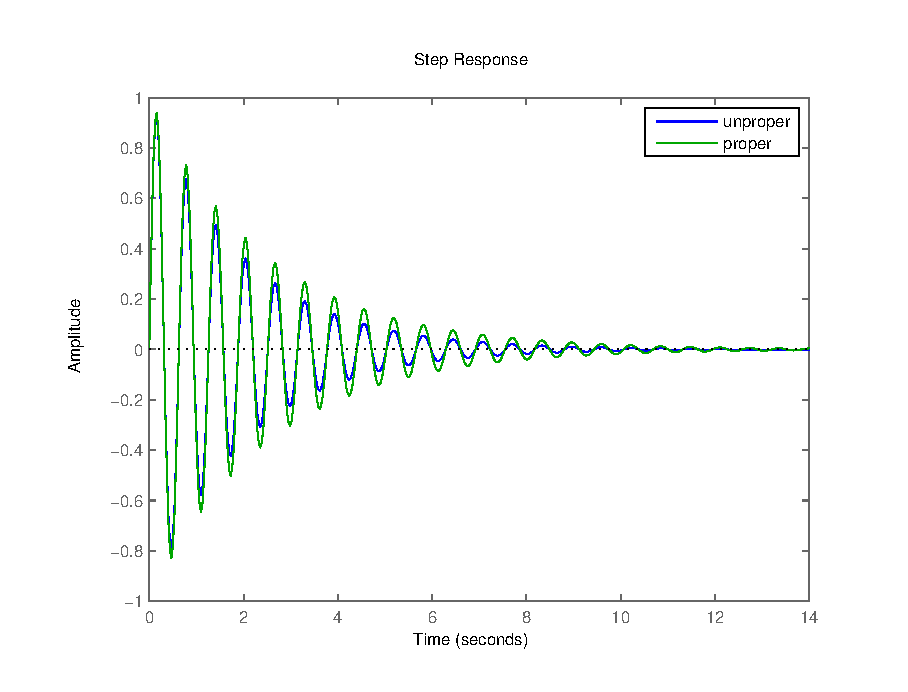
\includegraphics[width=\columnwidth]{fig/stepProper421.eps}
    \caption{Step response of the system with the proper \& unproper $F_y$} 
    \label{stepProper421}
\end{figure}


% \subsubsection{Exercise} 

Using Glover-MacFarlane controllers lead to a huge improvement of the controlled system:
\begin{shortitemize}
    \item All time are reduced (at least by a factor 2)
    \item Overshoots are decreased (at least by a factor 5)
    \item The step responses (non-minimum case) do not go in the wrong direction
\end{shortitemize}

% \subsubsection{Exercise} 

The main differences between the minimum phase case and the non-minimum phase case using Glover-MacFarlane controllers are (differencies are rather similar as the one using the decentralized controllers):
\begin{shortitemize}
    \item The non-minimum phase system is much slower (both for step response and disturbance rejection);
    \item Disturbances on the top tanks have more impact on the non-minimum phase system (whereas the perturbation on the lower tanks have a similar impact on both systems).
\end{shortitemize}


% \subsubsection{Exercise}

The two previous exercises lead to the design of the following controller:

$$F_r(s) = \frac{1}{1 + \tau s}$$
$$F_y(s) = K \frac{\tau_D s + 1}{\beta \tau_D s +1}\frac{s + \omega_I}{s} \frac{\omega_0^2}{(s+\omega_0)^2}G(s)^{-1} G_d(s)$$

With:

$$\begin{array}{rcl}
    \tau & = & 0.14 \text{ s}\\ 
    K &  = & 1.35\\
    \tau_D &  = & 0.078\text{ s}\\
    \beta &  = & 0.75\\
 \omega_I &  = & 5 \text{ rad.s}^{-1}\\
    \omega_0 &  = & 50 \text{ rad.s}^{-1}\\
\end{array}$$

\textbf{All the criteria are met:}

\begin{shortitemize}
    \item Rise time:
        $$t_r \leq 0.20\text{s}$$
    \item Overshoot:
        $$D(\%) \leq 10\%$$
    \item Step in the disturbance:
        $$|y(t)| \leq 1, \forall t \text{ and } |y(t)| \leq 0.1, \forall t \geq 0.5\text{ s}$$ 
    \item Control signal obeys:
        $$|u(t)| \leq 1, \forall t$$
\end{shortitemize}

Figure \ref{designFr} shows the step response of the system, the response to a step in the disturbance and the bode diagram of the sensitivity and complementary sensitivity functions.

\begin{figure}[h!t]
    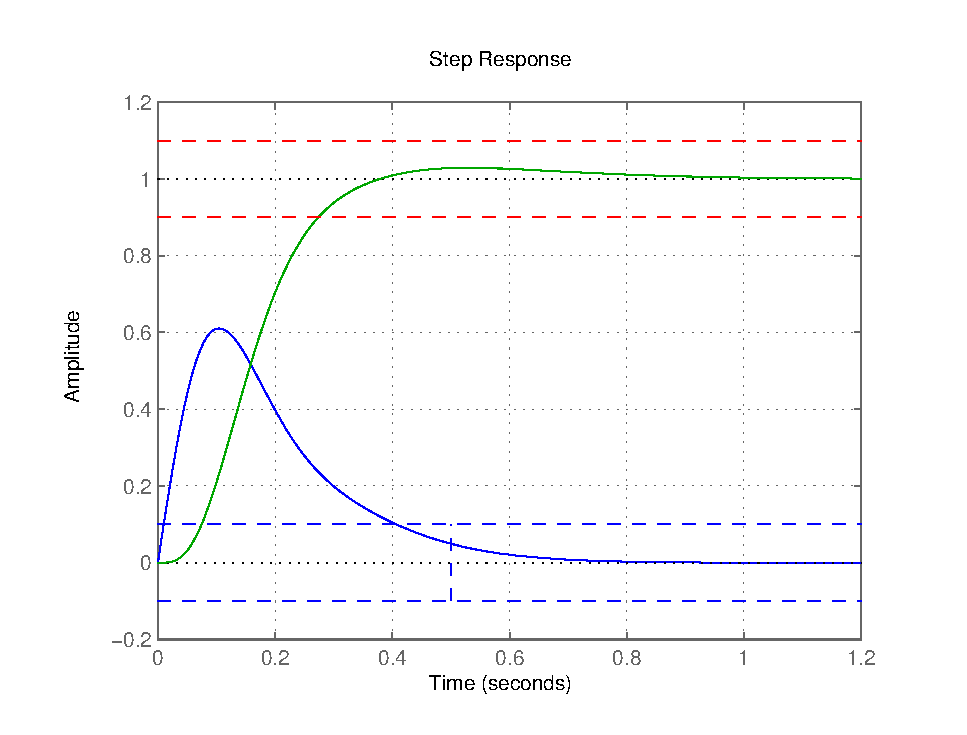
\includegraphics[width=\columnwidth]{fig/designFr.eps}
    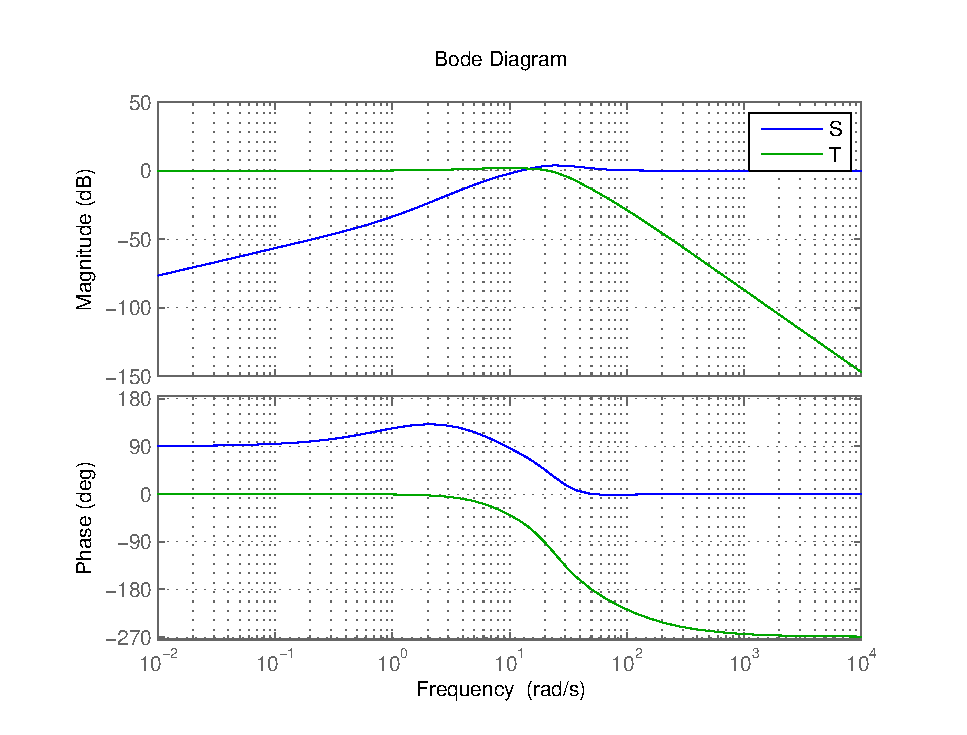
\includegraphics[width=\columnwidth]{fig/sensitivitiesFunction.eps}
    \caption{Step response of the system (green) and response to a step in the disturbance (blue) with the addition of the lead-controller \\ Bode diagram of the sensitivity and complementary sensitivity functions}
    \label{designFr}
\end{figure}




\end{document}
